\section{Time Analysis}

\subsection{End-to-End Latency}
The user experiences the sum of all sequential steps until the first byte of the response. Figure~\ref{fig:latency_timeline} illustrates the sequential stages and typical order of magnitude for each. There is no streaming: the client waits for the full list of messages (each with audio and lip-sync data) before playback.

\begin{itemize}
    \item \textbf{Default-message branch}: Fast (disk reads only) when no API keys or empty input.
    \item \textbf{OpenAI chain}: Loading the party program and building the chain add one file read and chain construction per request. The dominant cost is the single LLM call (e.g.\ GPT-4o-mini), typically on the order of 1--5 seconds depending on input and model.
    \item \textbf{Lip-sync stage}: For $n$ messages (up to 3), TTS runs in parallel but the stage is blocked until \emph{all} TTS finish. Then ffmpeg (MP3$\to$WAV) and Rhubarb run per message, again in parallel. So total time is roughly: $\max(\text{TTS}_1,\ldots,\text{TTS}_n) + \max(\text{ffmpeg+Rhubarb}_1,\ldots,\text{ffmpeg+Rhubarb}_n)$. Each ElevenLabs call can be 1--4 seconds; ffmpeg and Rhubarb add roughly 0.5--2 seconds per message depending on length. With three messages, the lip-sync phase alone can reach several seconds.
\end{itemize}

\begin{figure}[H]
\centering
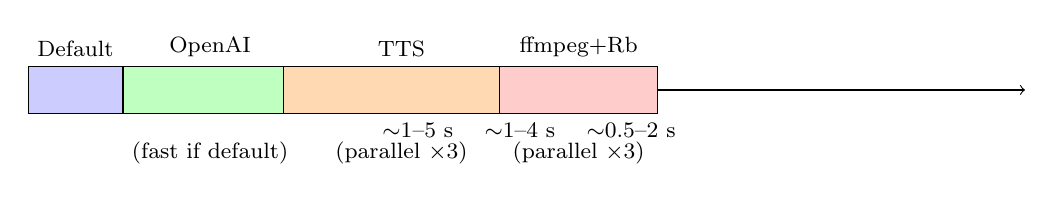
\begin{tikzpicture}[x=0.9cm, y=0.6cm, block/.style={rectangle, draw, minimum height=0.6cm, font=\small}]
    \draw [->] (0,0) -- (14,0);
    \node [block, fill=blue!20, minimum width=1.2cm] at (0.6,0) {};
    \node [above, font=\footnotesize] at (0.6,0.5) {Default};
    \node [block, fill=green!25, minimum width=2.2cm] at (2.5,0) {};
    \node [above, font=\footnotesize] at (2.5,0.5) {OpenAI};
    \node [block, fill=orange!30, minimum width=3cm] at (5.2,0) {};
    \node [above, font=\footnotesize] at (5.2,0.5) {TTS};
    \node [block, fill=red!20, minimum width=2cm] at (7.7,0) {};
    \node [above, font=\footnotesize] at (7.7,0.5) {ffmpeg+Rb};
    \node [below, font=\footnotesize] at (7, -0.5) {$\sim$1--5 s \quad $\sim$1--4 s \quad $\sim$0.5--2 s};
    \node [below, font=\footnotesize] at (2.5,-0.9) {(fast if default)};
    \node [below, font=\footnotesize] at (5.2,-0.9) {(parallel $\times$3)};
    \node [below, font=\footnotesize] at (7.7,-0.9) {(parallel $\times$3)};
\end{tikzpicture}
\caption[Latency timeline]{Typical latency breakdown: sequential stages with indicative durations (Rb = Rhubarb). No overlap between stages.}
\label{fig:latency_timeline}
\end{figure}

\begin{figure}[H]
\centering
\begin{tikzpicture}[node distance=1.2cm, block/.style={rectangle, draw, fill=blue!15, rounded corners, minimum height=0.65cm, font=\small}]
    \node [block, minimum width=1.8cm] (phase1) {TTS phase};
    \node [block, right=2.2cm of phase1, minimum width=1.8cm] (m1) {Msg 1};
    \node [block, below=0.35cm of m1] (m2) {Msg 2};
    \node [block, below=0.35cm of m2] (m3) {Msg 3};
    \node [block, below=1.4cm of phase1, minimum width=1.8cm] (phase2) {Phoneme phase};
    \node [block, right=2.2cm of phase2, minimum width=1.8cm] (p1) {Msg 1};
    \node [block, below=0.35cm of p1] (p2) {Msg 2};
    \node [block, below=0.35cm of p2] (p3) {Msg 3};
    \draw [->, thick] (phase1) -- (m1); \draw [->] (phase1) -- (m2); \draw [->] (phase1) -- (m3);
    \draw [->, thick] (m1) -- (phase2); \draw [->] (m2) -- (phase2); \draw [->] (m3) -- (phase2);
    \draw [->, thick] (phase2) -- (p1); \draw [->] (phase2) -- (p2); \draw [->] (phase2) -- (p3);
    \node [right=0.1cm of m3, font=\footnotesize] {parallel};
    \node [right=0.1cm of p3, font=\footnotesize] {parallel};
    \node [left=0.05cm of phase2, font=\footnotesize, align=right] {blocked until\\all TTS done};
\end{tikzpicture}
\caption[Lip-sync ordering]{Lip-sync stage: all TTS calls run in parallel, then all phoneme (ffmpeg + Rhubarb) runs in parallel. The second phase cannot start until the first fully completes.}
\label{fig:lipsync_ordering}
\end{figure}

\subsection{Weaknesses in Time}
\begin{enumerate}
    \item \textbf{Strictly sequential stages}: Default check $\to$ OpenAI $\to$ lip-sync. No overlap between LLM and TTS.
    \item \textbf{No streaming}: The frontend cannot start playing the first message while the rest are still being generated or synthesised.
    \item \textbf{Redundant work per request}: Party program and chain are re-built or re-loaded every time; only the chain reference is cached, not the result of \texttt{loadPartyProgram()} inside \texttt{getOpenAIChain()}.
    \item \textbf{STS path extra cost}: Speech path adds WebM$\to$MP3 conversion (file write, ffmpeg, read) and a Whisper API call before the same pipeline, increasing latency by 1--3 seconds.
    \item \textbf{Temp files}: Whisper and audios use temp files; cleanup is done in the happy path, but not guaranteed on early errors.
\end{enumerate}
